\section{Caso de estudio: Oficina de Relaciones Internacionales de la Facultad de Filosofía y Letras de la Universidad de Granada}

Para poder realizar un trabajo efectivo y poder tener en cuenta todas las necesidades, hemos de hacer un previo análisis sobre el caso que nos ocupa. Es por ello por lo que tenemos que comprender cuál es su labor, qué servicios prestan al estudiantado, al profesorado, de qué herramientas disponen, cuáles son sus necesidades y 

\subsection{Sobre la oficina}
La labor principal de la oficina es encargarse de la gestión de los programas de intercambio y la movilidad de los estudiantes e incluso de profesores. Como no podía ser de otra manera, proporcionan la información necesaria para los interesados en estos programas, tanto de fuera de la UGR como desde universidades extranjeras. Es más, también revisan convenios existentes con éstas y hacen otros nuevos para ofrecer cada vez más alternativas para poder mejorar nuestra formación.

En su día a día, atienden peticiones y dudas de los estudiantes que participan en alguno de los citados programas; es más, se dedican a asesorar y mostrar todas las alternativas de las que disponen cuando se nos presenta alguna situación complicada, de modo que podamos resolverlo de la forma en que más nos beneficie. Trabajan, en definitiva, con el futuro de los estudiantes, pues la movilidad la desarrollamos con el objetivo de complementar nuestra formación, algo fundamental y abrumador al mismo tiempo cuando se cruzan fronteras y se quiere seguir en el camino de la educación en una universidad que no es la de casa.

La oficina se sitúa junto a la secretaría, en la Facultad de Filosofía y Letras de la Universidad de Granada, en el Campus de Cartuja, y en ella trabajan alrededor de cuatro personas. Es, dadas las cifras que se tienen, una gran cantidad de información las que tan sólo unas pocas personas tienen que manejar con una herramienta que ha sido creada sobre la marcha para facilitar su importante labor; un trabajo que no puede parar ni tolera fallos, pues los estudiantes de movilidad son uno de los pilares fundamentales de la institución.

\subsection{Servicio al estudiantado}
\subsubsection{Estudiantes salientes o \textit{outcoming}}

En relación con los estudiantes salientes, en la oficina se encargan de coordinar a los tutores académicos, que son quienes revisan los acuerdos de estudios que los candidatos proponen para iniciar su movilidad. Una vez éstos les han dado el visto bueno, en la oficina revisan cada uno de los mismos para asegurarse de que todo está en orden. Una vez iniciada la movilidad puede darse el caso en que los estudiantes deseen hacer alguna modificación a su acuerdo, debido a algún cambio imprevisto o a que alguna asignatura no fuera como se esperaba, todo ello en el destino. En ese caso, el proceso sería el mismo: tendrían que volverse a revisar de nuevo los documentos para comprobar que todo está en orden.

También escuchan casos de estudiantes con problemas particulares y que deben ser examinados con detenimiento, para ofrecer la mejor alternativa, ya sea hablando con los coordinadores de los destinos internacionales o arreglando algún dato en los convenios que haya causado algún inconveniente en la movilidad de algún(a) estudiante. De este modo, las futuras movilidades podrán hacerse con una mayor posibilidad de éxito, sobre todo cuando se trate de convenios nuevos. Son múltiples los casos en que se deba necesitar asistencia: una lengua de impartición de las asignaturas distinta a la esperada, un nivel requerido en un idioma que no se había comunicado al estudiante, etc.

Una vez los estudiantes vuelven de su movilidad, se inicia el proceso de reconocimiento de créditos, para el cual se establecen unas correspondencias entre las calificaciones obtenidas en el destino y las que se van a especificar en su expediente en la UGR. Para ello, esta información debe estar reflejada en un documento oficial y que la secretaría pueda aceptar, por lo que en muchos casos el personal tiene que ponerse en contacto con los responsables en el destino y solicitar los certificados que sean precisos. De esta manera, se puede tener la certeza de que es alguien de confianza quien los remite, ya que se ha tomar muy en serio la veracidad de los mismos.

\subsubsection{Estudiantes entrantes o \textit{incoming}}

En cuanto a los \textit{incoming}, el proceso es distinto. Si bien es verdad que se les atiende para problemas similares a los que los estudiantes salientes podrían tener, este grupo viene a la UGR con un acuerdo de estudios previo ya hecho, de modo que es entonces cuando precisan del visto bueno extra de la Oficina, quien les confirma que las asignaturas a las que quieren acceder según lo que establezcan sus acuerdos de estudios tienen plazas disponibles. Es entonces cuando se podrían matricular de las mismas.

Este proceso es conocido como \gls{AM} en el ámbito de la movilidad y se hace de manera manual según las plazas que establece la facultad para cada asignatura. Es gracias a la ayuda de TWINS que puedan no sólo ver estas asignaciones de una mejor manera, sino que también tienen la posibilidad de generar los horarios para los estudiantes, algo fundamental y que les preocupa mucho cuando vienen a hacer su movilidad a la UGR. Pensemos que el simple hecho de que dos asignaturas tengan lugar en la misma hora supone un cambio inminente. Para ello, los interesados tienen que estudiar cuáles son las alternativas de que disponen, atendiendo al número de plazas restantes en las demás asignaturas, no dejando de lado si la franja horaria en la que se imparte clase es compatible con su horario final.

Como es lógico, tendrán que reportar estos cambios que hagan a sus universidades de destino tal y como éstas establezcan, pues al fin y al cabo el proceso para ellos será el mismo por lo general cuando vuelvan a casa.


\subsection{Servicios al profesorado (PDI)}

Al igual que los estudiantes, el Personal Docente Investigador tiene posibilidad de participar en programas de movilidad; es decir, hay convenios que contemplan la acogida del profesorado.

Es en la Oficina de Relaciones Internacionales de la facultad donde gestionan y registran estos convenios. Una vez hay constancia de ellos, el personal puede solicitar un programa al igual que los estudiantes; no obstante, es la ORI central quien se encarga de sus gestiones a lo largo de la movilidad. Esto es, no establecen una interacción directa con la oficina de la facultad.

En su caso no tienen un acuerdo de estudios, sino que tienen un acuerdo de movilidad o \textit{mobility agreement}, donde se pone de manifiesto la intención y los objetivos del/de la interesado/a con el programa que desea hacer.

%COMPROBAR SI HAY REGISTROS EN TWINS Y ACTUAR EN CONSECUENCIA 


\subsection{Coordinación con la Oficina de Relaciones Internacionales de la UGR}

Todo comienza cuando la ORI envía los datos de las adjudicaciones de las plazas de movilidad a la secretaría de la facultad. Es entonces cuando comienzan los trámites administrativos: se registra a cada estudiante de acuerdo a su destino para comenzar a confeccionar su expediente en base a su acuerdo de estudios, documentos firmados y demás información necesaria. Todo ello tendrá que quedar en conocimiento de la ORI una vez acabe la movilidad.

Establecen una estrecha comunicación también cuando se tratan asuntos económicos en relación a las becas. Con la confirmación de las fechas de llegada al destino y vuelta al origen se hace un contraste con la información presente en el convenio, que es otro acuerdo que los estudiantes se comprometen a cumplir. Se tiene en cuenta si el interesado/a ha realizado la movilidad durante la totalidad del periodo para la cual estaba prevista. De no ser así, la cantidad económica final tendrá que ser distinta a la prefijada para la ayuda a recibir por los estudiantes.

Por tanto, es de gran importancia guardar toda la información referente al proceso, pues al fin y al cabo la ORI tiene que coordinar que los distintos programas se están llevando a cabo sin incidencias, ya que, al fin y al cabo, es otro organismo asegurador del buen funcionamiento de esta alternativa al estudio continuado en la universidad que tanta importancia tiene hoy en día y que cada vez está más en auge.

\subsection{La base de datos TWINS}

%TWINS alberga actualmente unos 2055 registros de estudiantes desde el curso 2018-2019, incluyendo a algunos de ellos que han manifestado su intención de realizar un programa de movilidad en la Facultad de Filosofía y Letras durante el curso 2020/2021. 

TWINS alberga desde el curso 2018/2019 un volumen de datos que plasmamos en la tabla \ref{tab:estadisticasTWINS}. Al tratarse de una base de datos en la herramienta ofimática Microsoft Access\textregistered, la aplicación consta más bien de una simple capa a modo de interfaz que permite al usuario interactuar con la base de datos. La presentación de los datos se posibilita gracias a la ejecución de consultas preestablecidas (\textit{Query By Example}, QBE) que se almacenan y se indica en qué campos ha de mostrarse la información. Cuando se realiza alguna acción que requiera el borrado, inserción o actualización de registros se hace uso de las macros, que son trozos de código que disponen distintos flujos de información entre las tablas implicadas en dicha operación.

\begin{figure}
	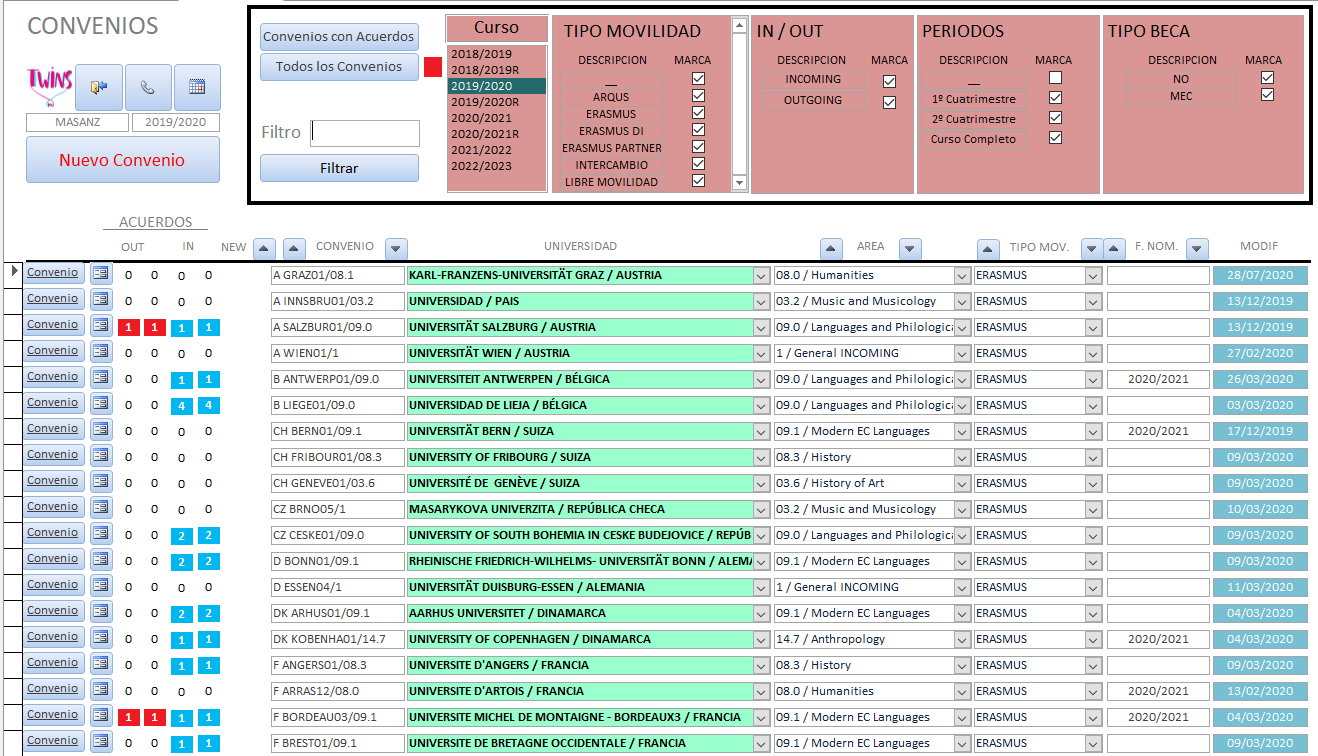
\includegraphics[width=\textwidth]{img/Capturas de TWINS/vistaConvenios.png}
	\caption[Convenios]{Vista de Convenios}
	\label{fig:vistaConvenios}
\end{figure}

\begin{table}[h]
	\begin{center}
		\begin{tabular}{ | c | c | } 
			\hline
			\multicolumn{2}{|c|}{\textbf{Administración}} \\
			\hline
			Estudiantes \footnotemark & 2055 \\ 
			\hline
			Tutores & 58 \\
			\hline
			Convenios  & 607 \\ 
			\hline
			Expedientes & 5049 \\ 
			\hline
			\multicolumn{2}{|c|}{\textbf{Base de datos}} \\
			\hline
			Tablas & 108 \\
			\hline
			Relaciones & 60 \\
			\hline
			Macros & 55 \\
			\hline
			Formularios & 152 \\
			\hline
			Consultas QBE & 343 \\
			\hline
		\end{tabular}
		\caption{Estadísticas de TWINS}
		\label{tab:estadisticasTWINS}
	\end{center}
\end{table}~
\footnotetext{Tanto \textit{incoming} como \textit{outcoming}}



\subsubsection{El modelo de datos}
\label{ModeloDatos}

El modelo relacional propuesto por Codd es el elegido para el diseño de esta base de datos. Las distintas tablas de la misma se conectan mediante relaciones que establecen restricciones para mantener la consistencia entre los datos.

Las tablas son una forma característica de almacenamiento de este modelo, en contraposición con otras disposiciones de la información usadas por otros sistemas y que, al fin y al cabo, se diseñan de otro modo porque se han de satisfacer unas necesidades distintas.

En este caso, podemos entender que la herramienta TWINS fue creada en Access y, por tanto, en un modelo de datos relacional dado el fácil acceso al usuario no experto en la materia, facilitando la operatividad con las bases de datos.

Es, sin duda, el modelo que más se utiliza aún hoy en día, el cual promete una determinada efectividad siempre y cuando el volumen de información a manejar no sea excesivamente elevado. En este caso, aunque la información que se requiere manipular en la oficina no es fácilmente manejable por personas, sí que aún podemos continuar utilizando este modelo para el desarrollo de la nueva herramienta twinX. Se entiende que no se tendrán más de unos 1000 estudiantes por curso académico (en una sola facultad) y que el número de convenios y tutores no será ni mucho menos parecido, considerando, eso sí, que la cantidad de \glspl{ExpedienteTWINS} será aproximadamente el doble que la de los estudiantes para los que se creen dichos registros.

Así pues, el modelo relacional parecer ser suficiente para las funcionalidades básicas y necesarias para trabajar en la oficina que twinX pretende implementar.

No obstante, no olvidemos la intención de extender la funcionalidad del actual TWINS para que los propios estudiantes puedan dejar atrás el constante envío de documentos entre sus tutores académicos por correo electrónico, de modo que puedan dar el salto a una plataforma que implemente una interfaz que les permita prescindir de estos documentos, como el acuerdo de estudios, y trabajar con la información directamente (aunque se posibiliten las conversiones a certificados que puedan ser impresos). En este contexto, se ha de tener en cuenta la forma de tratar los datos que se quiere realizar, que tendrá que adaptarse a este modelo de datos que va a ser usado también en twinX.

%Si todas las asignaturas de la universidad de origen se tienen en memoria y tan sólo se tienen que registrar las de la universidad de destino, tan sólo tendríamos que guardar códigos, órdenes y los nuevos nombres para esas asignaturas. Sin embargo, si esto se complicara y tuviéramos que almacenar documentos, quizás, para esa parte de la aplicación, sería conveniente estudiar la posibilidad de implementar una base de datos cuyo modelo de datos esté enfocado a la búsqueda de estos y, no menos importante, optimizado para dicho propósito, algo que sería impensable en una base de datos relacional. Un ejemplo de estas bases de datos es \textbf{Elasticsearch}, que permite hacer búsquedas complejas en texto, a través de datos estructurados y desestructurados. Esta podría ser una buena opción a utilizar una vez se alcance una determinada complejidad en el sistema de almacenamiento, pero en nuestro caso, solo lo comentamos como posibles trabajos futuros.

\subsubsection{Funciones implementadas}

\begin{itemize}
	\item \textbf{Funcionalidades básicas}\\
	Entre las funciones que hacen que TWINS cobre sentido, destacamos las siguientes:
	
	\begin{itemize}
		\item \textbf{Almacenamiento de información administrativa:} estudiantes, tutores, convenios, expedientes, etc.
		\item \textbf{Asociación de estudiantes con otras entidades:} estudiantes con su tutor, el convenio respecto del cual realizan su movilidad, sus expedientes, etc.
		\item \textbf{\gls{AM}}: para poder organizar a los estudiantes \textit{incoming}
		\item \textbf{Envío masivo de correos electrónicos:} posibilita funciones como las \glspl{Nominacion} automáticas o la comunicación a los participantes en los programas de movilidad de su tutor académico.
		\item \textbf{Generación de documentos automática:} disposición de los distintos datos en documentos que son entregables a estudiantes para mostrarles un sumario de su situación académica
		\item \textbf{Creación, edición y borrado de los datos dentro de la aplicación}
		\item \textbf{Anotación de futuras modificaciones a documentos ajenos a la oficina:} como son, por ejemplo, los convenios, que quedan registrados en la sede de la UGR y no pueden ser modificados hasta una fecha concreta, fuera del control de la oficina.
		\item \textbf{Recuperación de información de otros formularios externos a la aplicación:} para el registro de nuevos estudiantes (que es hasta ahora la mejor aproximación a la automatización de dicho proceso de la que se dispone) y, por ejemplo, para registrar datos de estudiantes afectados de alguna manera por la COVID-19.
	\end{itemize}

	\item \textbf{Funcionalidades específicas}\\
	Entre las que destacan la generación de informes con fines estadísticos para la oficina, información de asignaturas o menús para gestionar formularios creados por el personal para poder posteriormente transferir la información a la herramienta TWINS.
	
	También disponen de un sistema de alertas en relación con las tareas a realizar por el personal y con una especie de calendario donde se notifican los eventos temporales más próximos a atender.
\end{itemize}

\subsubsection{La interfaz de usuario}

Como hemos señalado en anteriores secciones, toda la aplicación yace sobre la herramienta de Microsoft\textregistered. Por ello, tanto los datos, como la presentación o vista y el control ejercido sobre los mismos no tiene separación alguna.

Al margen de esto y analizando las ventajas que el uso de Access\textregistered \ nos podría aportar, tenemos una manera de crear una interfaz de usuario de una manera más sencilla de lo normal. Tan sólo basta con arrastrar y redimensionar un botón con el ratón y una casilla para mostrar texto y con unas simples instrucciones tenemos una acción que, al pulsar el nuevo botón, en la casilla podría mostrarse, por ejemplo, cuántos registros almacena una determinada tabla (o varias de ellas) en la base de datos. Las consultas a la base de datos pueden almacenarse y reutilizarse según se quiera. A las interfaces se las conoce como \textbf{formularios} en Access\textregistered

También pueden programarse como si de una consulta se tratara, acciones que impliquen la modificación, borrado o creación de registros en la base de datos. A estas piezas de código funcionales se les da el nombre de \textit{macros}.

Una vez mencionadas las posibilidades funcionales, abordemos el uso de las mismas que han hecho para construir TWINS.

Lo primero que nos encontramos tras abrir la aplicación, es una pantalla de login con los distintos usuarios que pueden acceder al sistema (figura \ref{fig:login})

\begin{figure}
	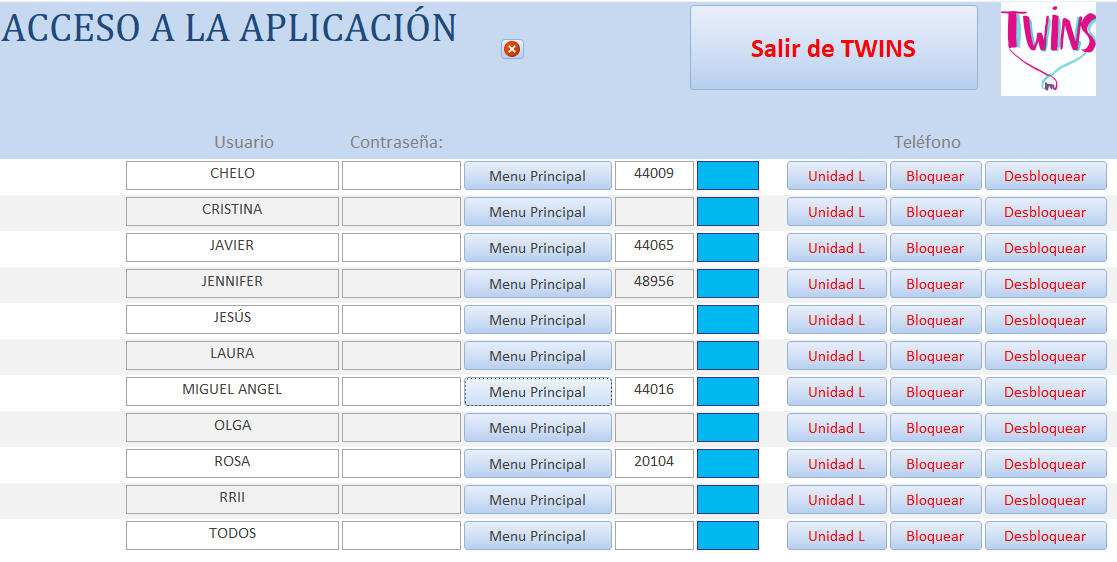
\includegraphics[width=\textwidth]{img/Capturas de TWINS/login.png}
	\caption[Login de TWINS]{Vista del login inicial de TWINS con todos los usuarios}
	\label{fig:login}
\end{figure}


Tras identificarnos, nos topamos, antes de llegar a la pantalla principal, con tres pantallas más:

\begin{itemize}
	\item El calendario (figura \ref{fig:calendario}) proporciona una vista genérica de todos los eventos que tienen lugar y que conciernen a la oficina o que tratan de asuntos relacionados con la misma. También se guardan plazos para realizar determinadas tareas. Los eventos del calendario\footnote{Nótese la especificación de « evento de calendario » o « \gls{EventoExpedienteTWINS} » en las definiciones correspondientes para establecer la diferenciación entre eventos que tienen que ver con la planificación en el calendario y los que componen los \glspl{ExpedienteTWINS}} son públicos a todos los usuarios de TWINS y en la creación de las entradas en él se permite establecer un(a) encargado/a de la tarea, de modo que de un vistazo puedan verse los avisos pendientes que se tienen para un determinado evento.
	
	\begin{figure}
		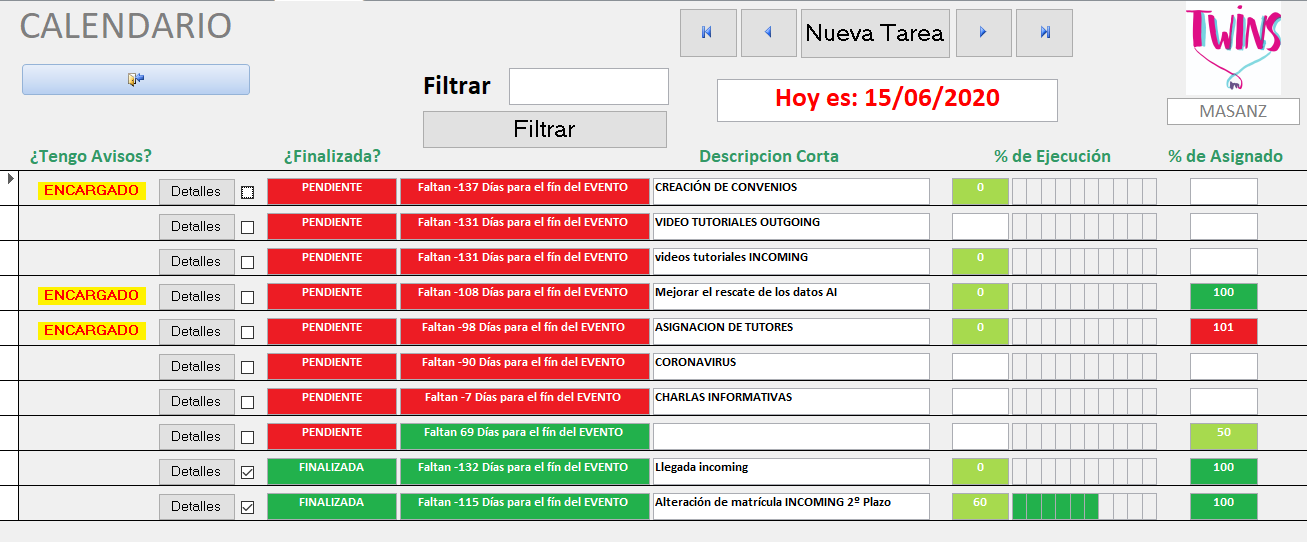
\includegraphics[width=\textwidth]{img/Capturas de TWINS/calendario.png}
		\caption[Calendario de TWINS]{Vista del calendario en TWINS con los eventos existentes y visibles por todos los usuarios}
		\label{fig:calendario}
	\end{figure}
	
	
	\item La pantalla de avisos (figura \ref{fig:avisos}) nos alerta de las acciones que tenemos que realizar con mayor urgencia, dado que han sido programadas para tenerlas listas para una fecha cercana y necesitan de la atención del usuario al que se notifica. Los avisos, al igual que un mensaje cualquiera, tienen emisor y receptor; es decir, hay alguien que los crea y los dirige a otra persona. Cuando se añade un evento al calendario, se especifican ambos actores, de modo que cuando está próxima la fecha de alguna tarea, se crea el aviso y notifica a aquel al cual le ha sido asignada. Normalmente, un usuario solo puede visualizar los avisos que le han sido dirigidos, salvo el superusuario, quien puede ver todos los avisos de todos los usuarios aparte de los propios
	
	Por supuesto, también se pueden crear avisos fuera del contexto de los eventos de calendario, lo que también implica la existencia de emisor, receptor y fecha de caducidad. Al margen de la importancia que se le da a la notificación del número restante de días para que una tarea caduque, esta última forma de hacer uso de los avisos podría verse como imaginando al creador, en la oficina, dejando una nota adhesiva en la mesa de su compañero/a.
	
	 \begin{figure}
	 	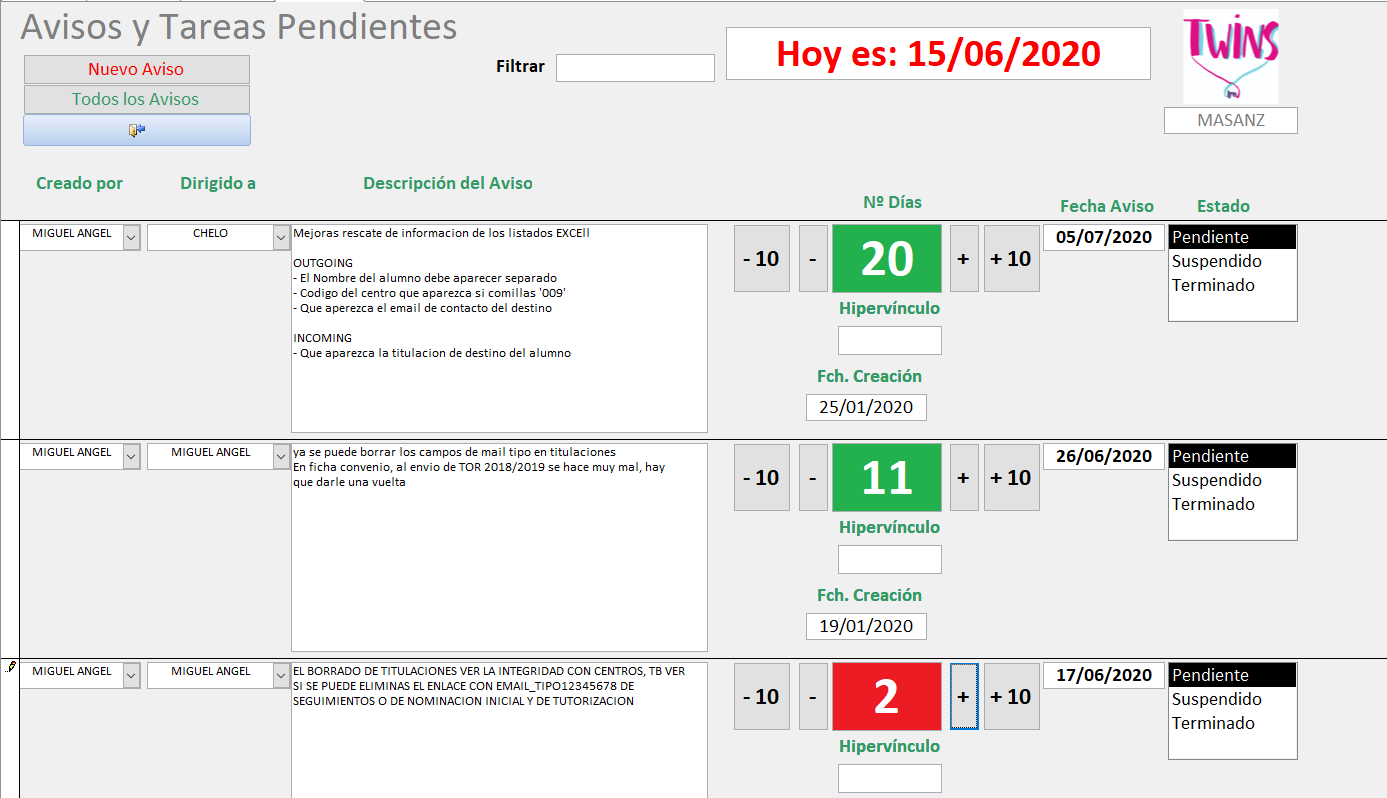
\includegraphics[width=\textwidth]{img/Capturas de TWINS/avisos.png}
	 	\caption[Avisos de TWINS]{Vista de los avisos en TWINS desde el usuario administrador}
	 	\label{fig:avisos}
	 \end{figure}
	 
	
	\item Dejando atrás los plazos y los eventos del calendario, otro elemento de gran importancia y con lo que trabajan día a día en la oficina (y no sólo en un cierto momento del cuatrimestre académico) son los \glspl{EventoExpedienteTWINS}. Pensemos que a diario surgen problemas, inconvenientes o simplemente hay que actualizar la situación de un estudiante. Por ello, la siguiente pantalla tras descartar las dos anteriores es la de eventos (de expediente) sin procesar (figura \ref{fig:eventosSinProcesar}).
	
	En ella, los usuarios de gestión pueden acceder a la información relacionada con el evento, como los demás eventos, los expedientes del alumno para el cual se está mostrando la información, o directamente las fichas del estudiante o el convenio en sí mismas.
	
	\begin{figure}
		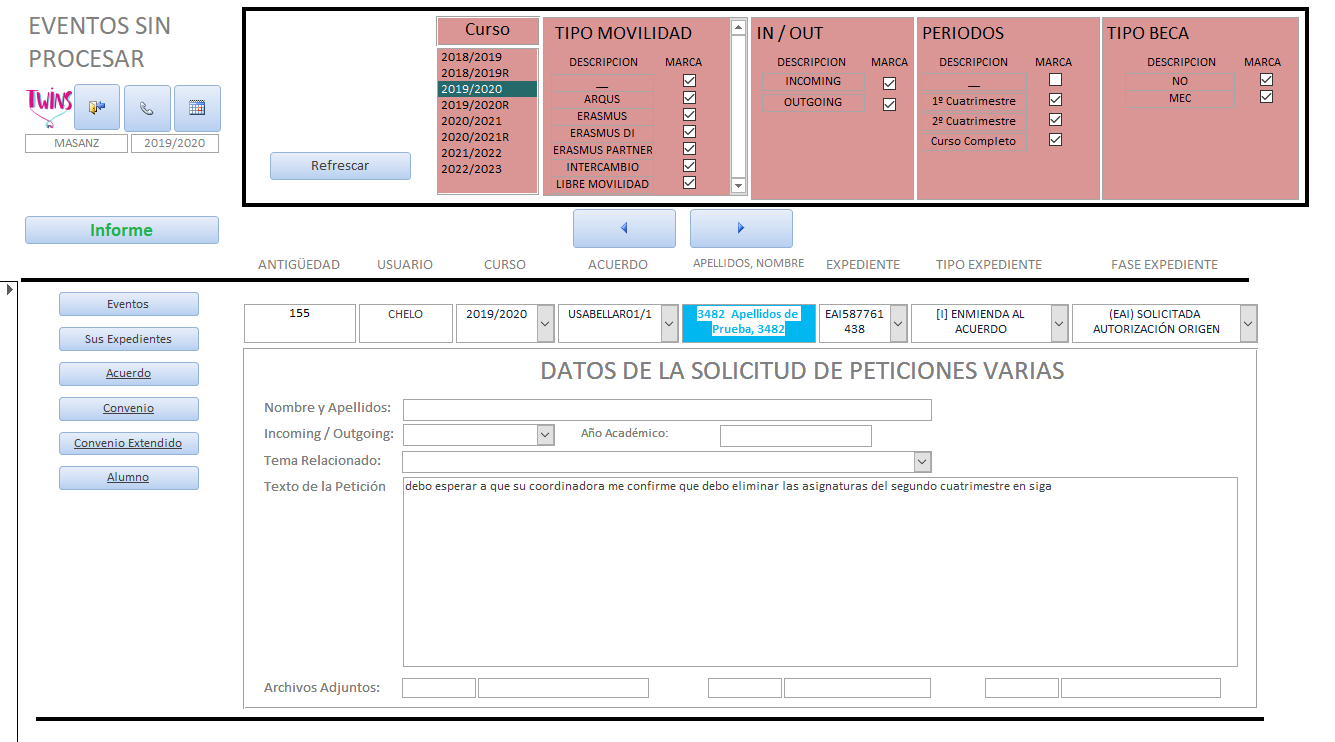
\includegraphics[width=\textwidth]{img/Capturas de TWINS/eventosSinProcesar.png}
		\caption[Eventos sin procesar de TWINS]{Menú de eventos sin procesar en TWINS, una pantalla donde los usuarios ven fácilmente el trabajo acumulado}
		\label{fig:eventosSinProcesar}
	\end{figure}
	
	
\end{itemize}

Finalmente, llegamos a la pantalla principal (figura \ref{fig:pantallaPrincipal}), de donde parten todos los menús (incluso los que acabamos de ver, que se muestran automáticamente identificarse correctamente en el sistema). En ella, no vemos ninguna información como la presentada en capturas anteriores (ni indicador de notificaciones, mensajes o alertas; nada). Lo que sí podemos apreciar es una selección en la cabecera de la vista principal con la que se filtrará el contenido que aparezca tras acceder a cualquier elemento del menú. Esto es, al solicitar determinada información cuando entremos a cierto menú, sólo se nos mostrarán aquellos datos que estén especificados en dicho cuadro de filtrado. Así, las consultas que se pueden hacer a la base de datos son mucho más cómodas y accesibles a todos los usuarios que no tienen por qué tener conocimiento de estos sistemas.

\begin{figure}
	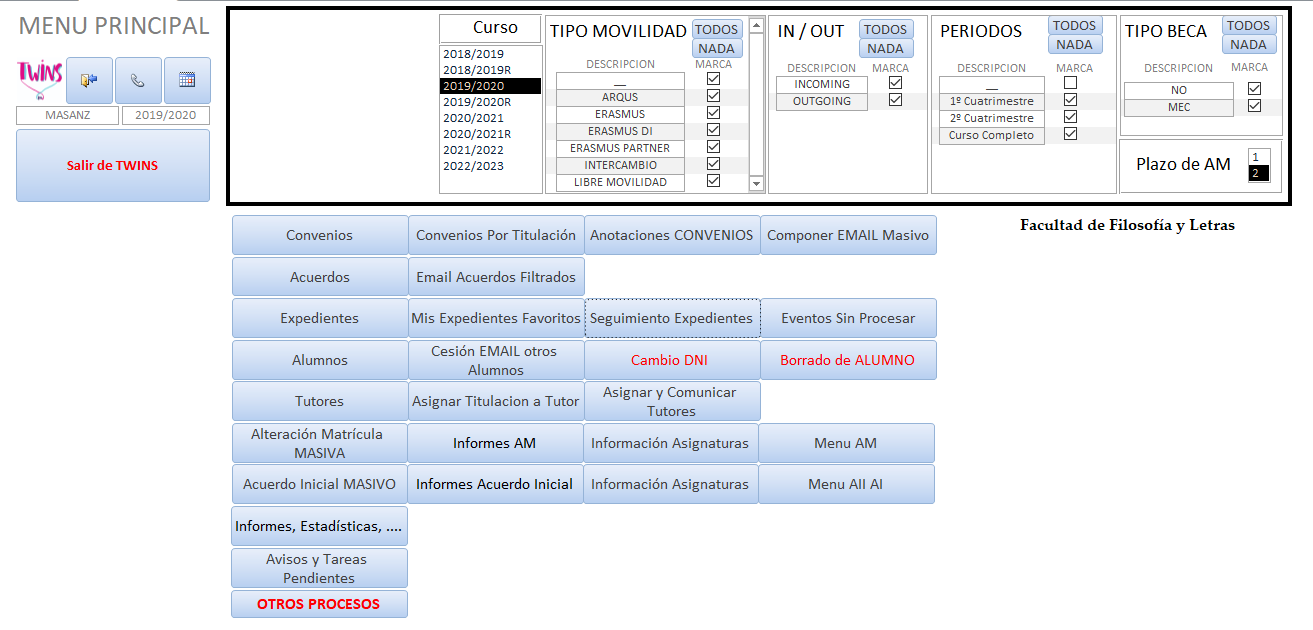
\includegraphics[width=\textwidth]{img/Capturas de TWINS/pantallaPrincipal.png}
	\caption[Menú principal de TWINS]{Pantalla principal de TWINS. Desde aquí podemos acceder a todos los menús anteriormente mostrados.}
	\label{fig:pantallaPrincipal}
\end{figure}

Si accedemos, por ejemplo, a la vista de convenios que ya hemos mostrado con anterioridad (figura \ref{fig:vistaConvenios}), el cuadro de filtrado se nos bloquea (ya hemos hecho una consulta y, para hacer otra, con otros parámetros, tendríamos que retroceder y volver a establecer nuestras preferencias de búsqueda). Se listan los convenios tal y como se han solicitado. El orden puede variarse a través de las flechas en las distintas columnas. Sin embargo y como es lógico, no se muestra toda la información de una tabla. Es más, realmente se están solicitando datos de distintas tablas (figura \ref{fig:tablasConsultaConvenios}). Este es un ejemplo de cómo la herramienta de creación de formularios de Access nos permite disponer la información de una tabla de forma más concisa que mostrando la tabla en crudo.

\begin{figure}
	\centering
	\includegraphics[width=\textwidth]{img/Capturas de TWINS/relaciónTablasConsultaConveniosLista.png}
	\caption[Tablas implicadas en consultar convenios en TWINS]{Relación de tablas implicadas en la consulta realizada para listar los convenios en TWINS}
	\label{fig:tablasConsultaConvenios}
\end{figure}

Si nos fijamos en las distintas entradas de la lista en la figura \ref{fig:vistaConvenios} de nuevo, correspondiente cada una a un distinto convenio, vemos que se tienen elementos como un botón para acceder al formulario de la vista del mismo, los estudiantes \textit{outcoming} o \textit{incoming} que están de movilidad según ese convenio, y demás elementos que son de relevancia para la entrada en concreto.

A efectos de diseño de la interfaz, es apreciable que ciertos campos de cada entrada se presentan con un elemento de lista, también conocido como \textit{dropdown}. No son editables hasta que no se accede a la vista del convenio, en contra de lo que puede dar a entender. Si generalizamos al resto de la aplicación, existen numerosos elementos con una disposición extraña como la que mencionamos, de modo que resultan atípicos para el usuario inexperto, lo que podría llevar a confusiones y una pérdida de confianza en el usuario que interactúe con el sistema, a pesar de que no habrá gran cantidad de gente que comience a utilizar el sistema por primera vez de forma avanzada como es la labor del personal de secretaría, quienes sí lo harán. De todos modos, no podemos dar nada por hecho y la labor de un experto en informática es, en esencia, facilitar y mejorar.

Es por ello por lo que gran parte de este proyecto se enfocará al rediseño de la aplicación de TWINS basado en técnicas de usabilidad. Esto será posible gracias a la aplicación de metodologías actuales y la realización de pruebas reales con usuarios que interaccionarán con el sistema.

En las figuras \ref{fig:cambioDNI}, \ref{fig:alumnos}, \ref{fig:cesionDeDatos} y \ref{fig:infoAsignaturas} se proporcionan otras vistas relativas a la interfaz de usuario. Podemos apreciar cómo se destacan con colores más llamativos los menús donde una acción indebida podría desenvolver acciones indeseadas. También, como elemento en común cada vez que aparece el nombre de los estudiantes, se marca en rojo si es \textit{outcoming} o en azul si, por el contrario, es \textit{incoming}. Aparte de esto, no comentaremos sus aspectos específicos, dado que la metodología empleada para su creación es la misma que ya hemos expuesto y la interacción por parte del usuario es similar. Nótese que no se muestran datos con carácter sensible debido a cuestiones de protección de datos.


\begin{figure}
	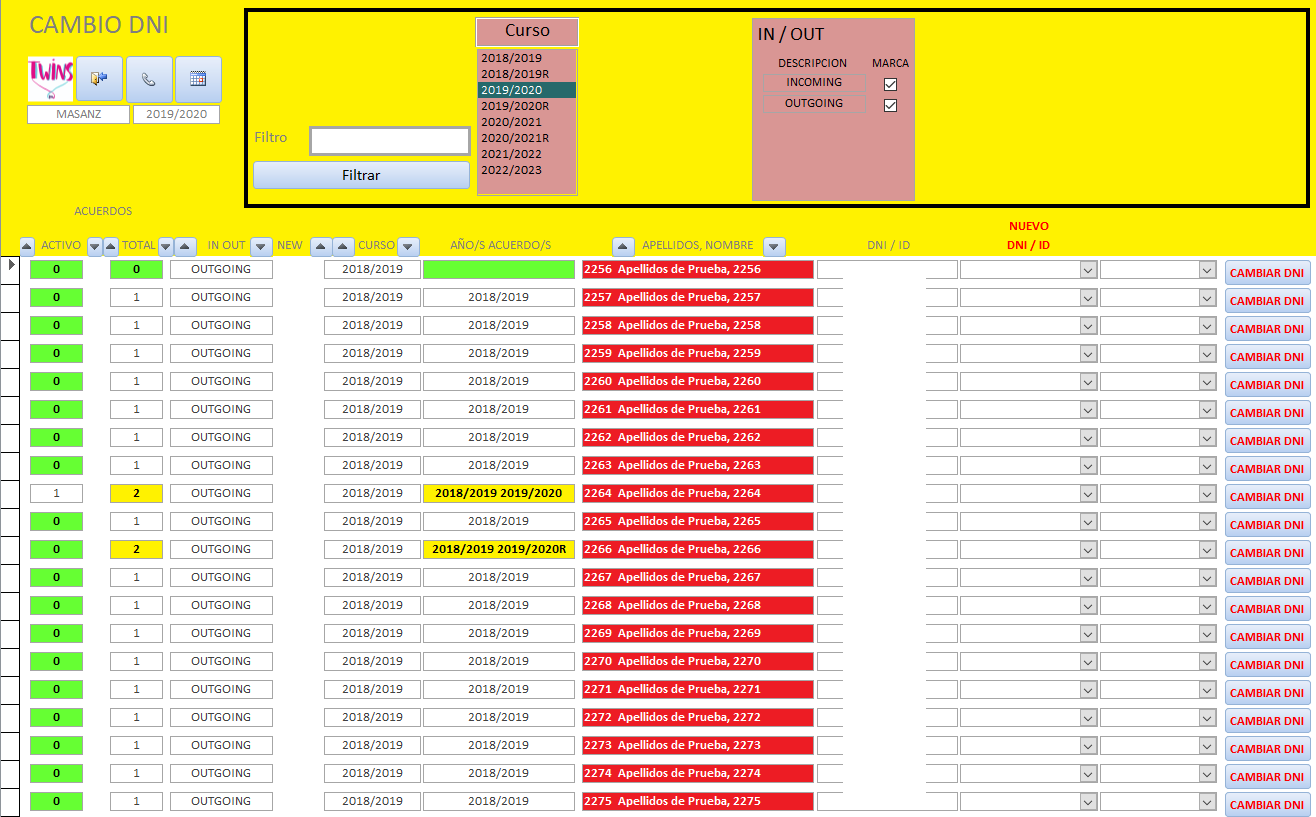
\includegraphics[width=\textwidth]{img/Capturas de TWINS/cambioDNI.png}
	\caption[Menú de cambio de DNI]{También existe en TWINS un menú específico para el cambio de DNI}
	\label{fig:cambioDNI}
\end{figure}

\begin{figure}
	\subcaptionbox{Vista de alumnos en TWINS \label{fig:alumnos}}{
		\centering
		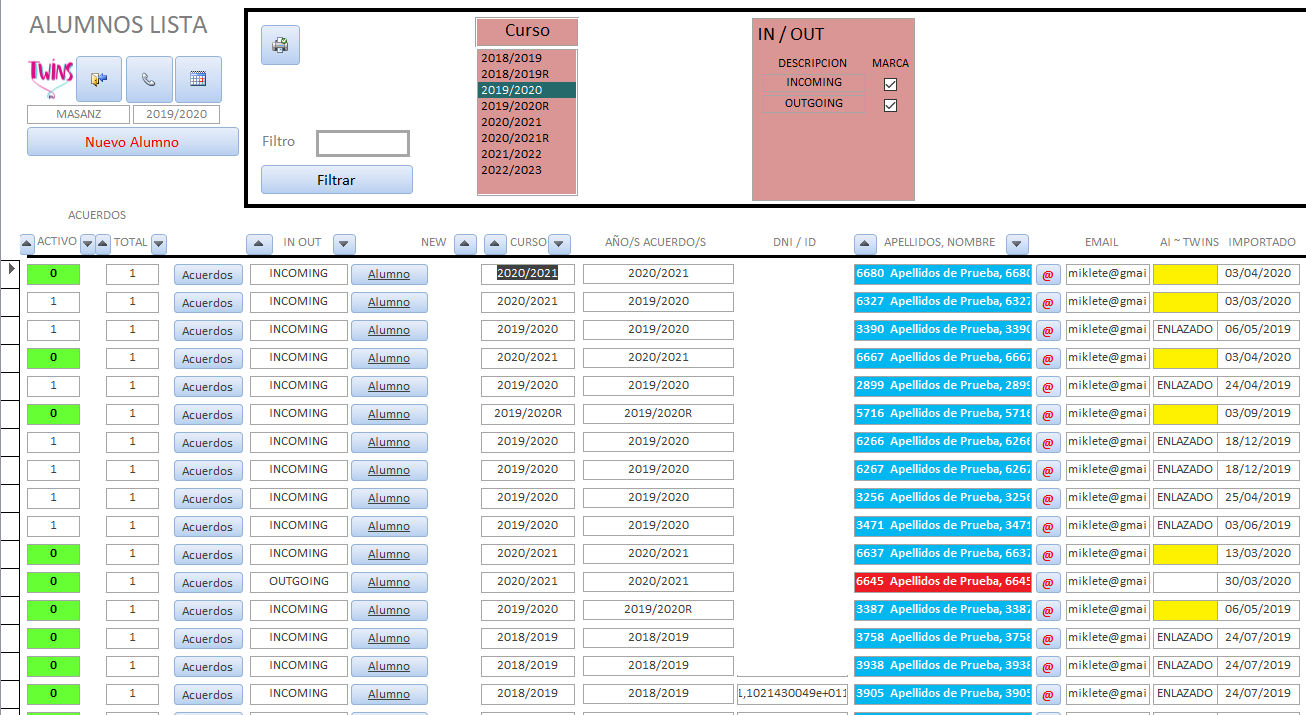
\includegraphics[width=\textwidth]{img/Capturas de TWINS/alumnos}
		
	}\par\medskip

	\subcaptionbox{Menú de gestión del consentimiento de cesión de datos de los estudiantes salientes en TWINS \label{fig:cesionDeDatos}}{
		\centering
		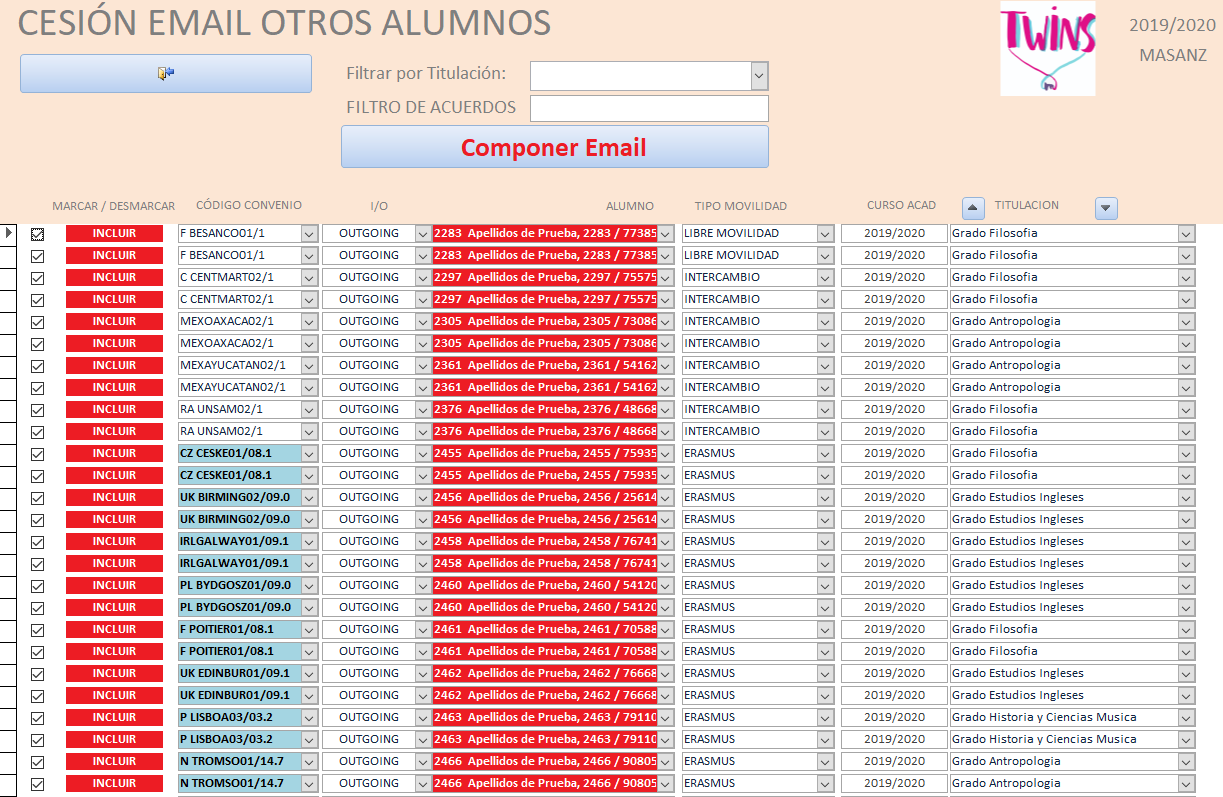
\includegraphics[width=\textwidth]{img/Capturas de TWINS/cesionDeDatos}
	} \par\medskip
\end{figure}

\begin{figure}
	\ContinuedFloat
	\subcaptionbox[Vista de información de asignaturas]{Menú de información de las asignaturas en TWINS (en la universidad local, de destino, de cara a los estudiantes entrantes) \label{fig:infoAsignaturas}}{
		\centering
		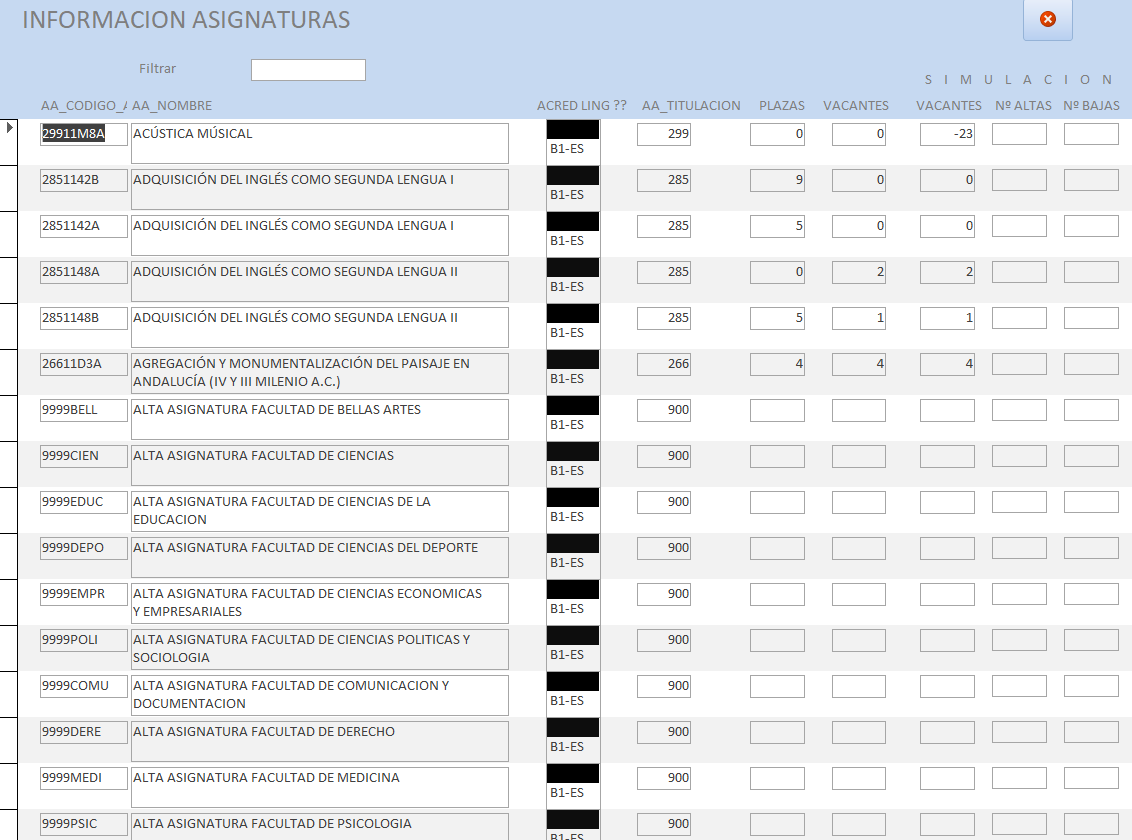
\includegraphics[width=\linewidth]{img/Capturas de TWINS/infoAsignaturas}
	}

\label{fig:adicionales}
\caption{Capturas adicionales de TWINS}

\end{figure}

\subsection{Estudio de necesidades de la Oficina de Relaciones Internacionales}

En general, la Oficina de Relaciones Internacionales de la facultad dispone de una herramienta que, dado que ha sido creada por un integrante de la secretaría de la facultad con una estrecha relación laboral con los miembros de la oficina, ha sabido cumplir los requisitos  operacionales del servicio. Muchas funcionalidades de la misma son muy concretas a las necesidades de la oficina (informes imprimibles con documentación específica, estadísticas, pegatinas para fundas de plástico, etc.)

No obstante, debido a las limitaciones de la metodología escogida para posibilitar estas gestiones, se ha llegado a un punto en que es muy complicado realizar modificaciones y extensiones a la misma, entre las que podemos destacar la existencia de un portal directamente conectado a la aplicación principal que posibilite la realización de gestiones por parte de los estudiantes. De este modo, tanto el estudiante como el personal de secretaría ahorrarían tiempo y su interacción no sería íntegramente en el correo electrónico. Esto es también extensible al papel de los tutores académicos.

Actualmente se ha hecho uso de herramientas auxiliares como los Formularios de Google\textregistered \ que permiten volcar datos al formato de hoja de cálculo, con lo que permite a TWINS reconocer la información y que pueda, a través de macros, crear nuevos registros en la base de datos para almacenarlos. Sin embargo, se precisa de la interacción humana para dicha tarea, al igual para muchas otras que se puedan querer automatizar o adaptar, como por ejemplo:

\begin{itemize}
	\item \textbf{Adaptar la mensajería} e implementarla dentro de la aplicación para llevar un mejor control de los casos de los estudiantes.
	\item \textbf{Automatización del seguimiento de las nominaciones} teniendo un portal externo donde otras universidades puedan nominar a sus estudiantes en la UGR.
	\item \textbf{Portal con vista para el estudiante entrante}, posibilitando que haga su propio registro en la plataforma y pueda ver su información en ella.
\end{itemize}

Al margen de las nuevas características a incluir, no podemos dejar de lado la necesidad de reconstruir un sistema desde cero, para que sea consistente, estable, con alta disponibilidad y fiabilidad y que pueda adaptarse a las necesidades tanto del personal de la oficina como a las del estudiantado. Es por tanto por lo que debemos descartar seguir utilizando la herramienta de Access\textregistered \ por sus limitaciones, expuestas en la sección ~\ref{ModeloDatos}.